\bluepage{Konfigurace Vertex Pulleru/Vertex Array Object}

\begin{frame}\frametitle{Vertex Array Object}
\scriptsize
\begin{itemize}
  \item Vertex Array object (VAO) contains configuration of vertex assembly unity (vertex specification / vertex puller).
  \item Vertex Assembly unit reads data from buffers and fills vertex attributes.
  \item VAO specifies connection of buffers and vertex shader input variables.
  \item It is required (even empty VAO).
  \item It can contains index buffer.
  \item Offset, stride, attrib size, type, ...
\end{itemize}

\begin{itemize}
  \item Vertex Array Object (VAO) obsahuje konfiguraci Vertex Assembly jednoty.
  \item Vertex Assembly jednotka čte data z bufferů a plní je do vstupních proměnných ve vertex shaderu.
  \item VAO obsahuje nastavení propojení shader programu a bufferů.
  \item V novějších verzích OpenGL je povinný.
  \item Obsahuje sadu nastavení pro každý vertex attribut a nastavení pro indexový buffer.
  \item Jeden vertex attribut je napojen na jednu vstupní proměnnou ve vertex shaderu.
  \item Mezi nastavení vertex attributu patří: číslo bufferu, velikost a typ datové položky, prokládání (stride), offset.
\end{itemize}
\end{frame}

\begin{frame}
\frametitle{Example - 0. invocation}
  \begin{figure}[h]
  \includegraphics[width=10cm,keepaspectratio]{pics/vao/puller0.pdf}
  \end{figure}
\end{frame}

\begin{frame}
\frametitle{Example - 1. invocation}
  \begin{figure}[h]
  \includegraphics[width=10cm,keepaspectratio]{pics/vao/puller1.pdf}
  \end{figure}
\end{frame}

\begin{frame}[fragile]
\frametitle{VAO - example}
{\tiny
\begin{minted}[bgcolor=bg]{packages/c_cpp.py:CppLexer -x}
GLuint vao;
glCreateVertexArrays(1,&vao);//vygenerovani jmena VAO

glVertexArrayAttribBinding(vao,0,0);
glEnableVertexArrayAttrib(vao,0);
glVertexArrayAttribFormat(vao,
  0,//attrib index
  2,//nof components (vec2)
  GL_FLOAT,//type
  GL_FALSE,//normalization
  0);//relative offset
glVertexArrayVertexBuffer(vao,0,
  vbo,
  (GLvoid*)(sizeof(float)*0),//offset
  sizeof(float)*5);//stride

glVertexArrayAttribBinding(vao,1,1);
glEnableVertexArrayAttrib(vao,1);
glVertexArrayAttribFormat(vao,1,3,GL_FLOAT,GL_FALSE,0);
glVertexArrayVertexBuffer(vao,1,vbo,(GLvoid*)(sizeof(float)*2),
  sizeof(float)*5);

glVertexArrayAttribBinding(vao,2,2);
glEnableVertexArrayAttrib(2);
glVertexArrayAttribFormat(2,4,GL_FLOAT,GL_FALSE,0);
glVertexArrayVertexBuffer(vao,2,vbo,(GLvoid*)(sizeof(float)*10),
  sizeof(float)*8);
\end{minted}
}
\end{frame}

\begin{frame}[fragile]
\frametitle{VAO}
  \begin{figure}[h]
  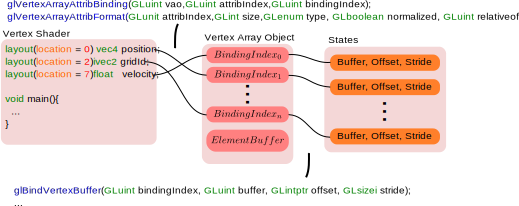
\includegraphics[width=11cm,keepaspectratio]{pics/vao/vao.pdf}
  \end{figure}
\end{frame}

